\documentclass[11pt, preprint]{article}
\usepackage{hyperref}
\usepackage{amsmath}
\usepackage{rotating}
 
\setlength{\footnotesep}{9.6pt}
\setlength{\parskip}{12pt}

\newcounter{thefigs}
\newcommand{\fignum}{\arabic{thefigs}}

\newcounter{thetabs}
\newcommand{\tabnum}{\arabic{thetabs}}

\newcounter{address}

\begin{document}

\begin{center}
  {\bf Radiative Processes in Astrophysics / Problem Set \#9 \\
    Due May 17, 2021}
\end{center}

\begin{enumerate}
\item Stars form in molecular clouds as the cooling of gas leads to
  fragmentation of cold cores and ultimately collapse into
  gravitational bound objects. A major sources of cooling is CO
  rotational line emission. You may wonder why it is CO and not the
  much more abundant H$_2$, and it turns out there are good reasons.

  \begin{enumerate}
    \item Estimate the energies and frequencies associated with the
      first rotational transition and the first vibrational transition
      of H$_2$. To make your life easier later, write down their
      scaling with the reduced mass of the molecule. Remember that
      $\Delta J=\pm 1$ are forbidden.
   \item What are the populations for the two upper states relative to
     the ground state if the populations are in thermodynamic
     equilibrium with the gas, for example through collisions?
   \item The Einstein $A$ coefficient for the $J~1$---$0$ transition
     in H$_2$ is $\sim 3\times 10^{-11}$ s$^{-1}$ and for the
     $v~$1---0 transition is $\sim 2.5\times 10^{-7}$ s$^{-1}$. Assume
     you are considering a cloud which is optically thin in these
     lines; then transitions from these upper states yield photons
     that escape the cloud and therefore cool the gas. Assuming the
     gas has a temperature $\sim 10$K, which kind of transition (from
     the first vibrational or first rotational state) will dominate
     the cooling?
   \item How long will it take for the gas to cool to $\sim 5$K, to an
     order of magnitude? Assume all the gas is in molecular hydrogen
     form.
   \item The Einstein $A$ coefficient for the $J~1$---$0$ transition in
     CO is $\sim 2\times 10^{-7}$ s$^{-1}$, and the typical (number)
     ratio of CO to H$_2$ is $6\times 10^{-5}$. How does the presence
     of CO change the cooling time? Assume only the first excited
     rotational state matters (this will underestimate the cooling
     rate by a factor two or so). 
  \end{enumerate}

\item Consider Figure \ref{fig:co}, which shows a spectrum which
  includes absorption from warm CO gas in our galaxy.
    Remember that CO's ground state is $\Sigma$, i.e. has no net orbital
    angular momentum of the electrons, it has no $\Delta J = 0$
    transitions during a rotational-vibrational transition.

  \begin{enumerate}
    \item Argue on the basis of the energies of these absorption lines that
      they involve vibrational transitions.
    \item The missing $Q$ branch location at the center locates the
      energy difference between two adjacent vibrational states (with
      $\Delta J = 0$. Assuming the Einstein $A$ coefficients do not
      depend very much on the particular rotational states involved,
      use the figure to make a very rough estimate of the temperature
      of the CO gas. 
  \end{enumerate}

\item Dust grains in the interstellar medium are heated by starlight
  and cool down through thermal emission.  They have some absorption
  efficiency $Q_{\rm a}(\nu)$ that defines how well they absorb at a
  given wavelength, which is also the efficiency with which they emit.
  \begin{enumerate}
  \item If the energy density of starlight is written as
    $u_{\nu\ast}(\nu)$, and the dust grains are spherical with a
    radius $a$, write the formula for the heating rate of a dust
    grain. This should involve an integral over $\nu$.
  \item What is the cooling rate due to thermal emission from the
    surface of the dust grain?
  \item If you assume that $Q_{\rm a}(\nu) =1$ (a constant), and
    $u_\ast = 10^{-12}$ erg cm$^{-3}$ (a typical value expected in the
    interstellar medium) then find the equilibrium temperature of the
    grains.
  \item In fact, $Q_{\rm a}(\nu) \propto \nu^{\beta}$, where
    $\beta\sim 1$--2 (actually it is more complicated than a power
    law). Do you expect the actual grain temperature to be larger or
    smaller than predicted in the previous question?
  \item Potentially collisions with gas particles could also heat the
    grains to the gas temperature (which is typically higher than the
    dust temperature---they are out of equilibrium for reasons that
    will become clear in this problem!). For a number density $n$ of
    some gas species at temperature $T_{\rm gas}$ estimate the rate of
    collisions with a dust grain of radius $a$. The average energy
    exchange should be $\sim k(T_{\rm gas} - T_{\rm dust})$ for a
    collision that is at least somewhat inelastic.  For the $u_\ast$
    given above, $T_{\rm gas} = 100$K, and $n=10$ cm$^{-3}$, what is
    the relative contribution of collisional and radiative heating?
    Explain why this means that the dust is not in thermodynamic
    equilibrium with the gas.
  \end{enumerate}

\end{enumerate}

      \begin{figure}[h!]
        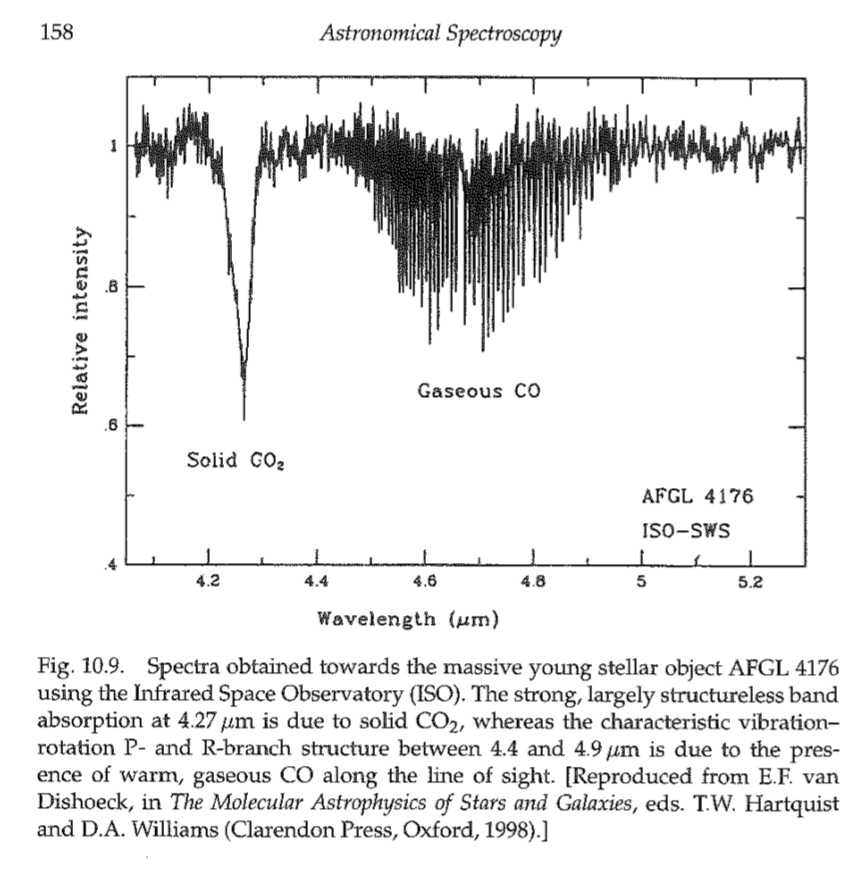
\includegraphics[width=0.9\textwidth]{tennyson-co-iso.jpeg}
        \caption{ \label{fig:co} From Tennyson, {\it Astronomical
            Spectroscopy} }
      \end{figure}

\end{document}

